%iffalse
\let\negmedspace\undefined
\let\negthickspace\undefined
\documentclass[journal,12pt,onecolumn]{IEEEtran}
\usepackage{cite}
\usepackage{amsmath,amssymb,amsfonts,amsthm}
\usepackage{algorithmic}
\usepackage{graphicx}
\usepackage{textcomp}
\usepackage{xcolor}
\usepackage{txfonts}
\usepackage{listings}
\usepackage{enumitem}
\usepackage{mathtools}
\usepackage{gensymb}
\usepackage{comment}
\usepackage[breaklinks=true]{hyperref}
\usepackage{tkz-euclide} 
\usepackage{listings}
\usepackage{gvv}                                        
%\def\inputGnumericTable{}                                 
\usepackage[latin1]{inputenc}     
\usepackage{xparse}
\usepackage{color}                                            
\usepackage{array}                                            
\usepackage{longtable}                                       
\usepackage{calc}                                             
\usepackage{multirow}
\usepackage{multicol}
\usepackage{hhline}                                           
\usepackage{ifthen}                                           
\usepackage{lscape}
\usepackage{tabularx}
\usepackage{array}
\usepackage{float}
\newtheorem{theorem}{Theorem}[section]
\newtheorem{problem}{Problem}
\newtheorem{proposition}{Proposition}[section]
\newtheorem{lemma}{Lemma}[section]
\newtheorem{corollary}[theorem]{Corollary}
\newtheorem{example}{Example}[section]
\newtheorem{definition}[problem]{Definition}
\newcommand{\BEQA}{\begin{eqnarray}}
\newcommand{\EEQA}{\end{eqnarray}}
\usepackage{float}
%\newcommand{\define}{\stackrel{\triangle}{=}}
\theoremstyle{remark}
\usepackage{ circuitikz }
%\newtheorem{rem}{Remark}
% Marks the beginning of the document
\begin{document}
\title{CH: Chemical Engineering}
\author{EE25BTECH11012 - BEERAM MADHURI}
\maketitle
\renewcommand{\thefigure}{\theenumi}
\renewcommand{\thetable}{\theenumi}

\begin{enumerate}

\section*{Q. 1--Q. 5 carry one mark each.}

\item The volume of a sphere of diameter 1 unit is\underline {\hspace{1cm}} than the volume of a cube of side 1 unit.
 \hfill{\brak{\text{CH 2016}}}
\begin{enumerate}
\begin{multicols}{4}
    \item least
    \item less
    \item lesser
    \item low
    \end{multicols}
\end{enumerate}

\item The unruly crowd demanded that the accused be \underline{\hspace{1cm}} without trial.
 \hfill{\brak{\text{CH 2016}}}
\begin{enumerate}
\begin{multicols}{4}
    \item hanged
    \item hanging
    \item hankering
    \item hung
    \end{multicols}
\end{enumerate}

\item Choose the statement(s) where the underlined word is used correctly:
\begin{enumerate}[(i)]
    \item A \underline{prone} is a dried plum.
    \item He was lying \underline{prone} on the floor.
    \item People who eat a lot of fat are \underline{prone} to heart disease.
\end{enumerate}
 \hfill{\brak{\text{CH 2016}}}
\begin{enumerate}
\begin{multicols}{4}
    \item (i) and (iii) only
    \item (ii) only
    \item (i) and (ii) only
    \item (ii) and (iii) only
\end{multicols}
\end{enumerate}

\item Fact: If it rains, then the field is wet.

Read the following statements:
\begin{enumerate}[(i)]
    \item It rains
    \item The field is not wet
    \item The field is wet
    \item It did not rain
\end{enumerate}
Which one of the options given below is \textbf{NOT} logically possible, based on the given fact?
 \hfill{\brak{\text{CH 2016}}}
\begin{enumerate}
\begin{multicols}{2}
    \item If (iii), then (iv).
    \item If (i), then (iii).
    \item If (i), then (ii).
    \item If (ii), then (iv).
    \end{multicols}
\end{enumerate}

\item A window is made up of a square portion and an equilateral triangle portion above it. The base of the triangular portion coincides with the upper side of the square. If the perimeter of the window is $6$ m, the area of the window in m$^2$ is \underline{\hspace{1cm}}.
 \hfill{\brak{\text{CH 2016}}}
\begin{enumerate}
\begin{multicols}{4}
    \item $1.43$
    \item $2.06$
    \item $2.68$
    \item $2.88$
    \end{multicols}
\end{enumerate}

\section*{Q.6--Q.10 carry two marks each.}

\item Students taking an exam are divided into two groups, $\mathbf{P}$ and $\mathbf{Q}$ such that each group has the same number of students. The performance of each of the students in a test was evaluated out of 200 marks. It was observed that the mean of group $\mathbf{P}$ was 105, while that of group $\mathbf{Q}$ was 85. The standard deviation of group $\mathbf{P}$ was 25, while that of group $\mathbf{Q}$ was 5. Assuming that the marks were distributed on a normal distribution, which of the following statements will have the highest probability of being TRUE?
 \hfill{\brak{\text{CH 2016}}}
\begin{enumerate}
\item No student in group $\mathbf{Q}$ scored less marks than any student in group $\mathbf{P}$.
\item No student in group $\mathbf{P}$ scored less marks than any student in group $\mathbf{Q}$.
\item Most students of group $\mathbf{Q}$ scored marks in a narrower range than students in group $\mathbf{P}$.
\item The median of the marks of group $\mathbf{P}$ is 100.
\end{enumerate}

\item A smart city integrates all modes of transport, uses clean energy and promotes sustainable use of resources. It also uses technology to ensure safety and security of the city, something which critics argue, will lead to a surveillance state.\\
Which of the following can be logically inferred from the above paragraph?
\begin{itemize}
\item [(i)] All smart cities encourage the formation of surveillance states.
\item [(ii)] Surveillance is an integral part of a smart city.
\item [(iii)] Sustainability and surveillance go hand in hand in a smart city.
\item [(iv)] There is a perception that smart cities promote surveillance.
\end{itemize}
\hfill{\brak{\text{CH 2016}}}
\begin{enumerate}
\begin{multicols}{2}
\item (i) and (iv) only
\item (ii) and (iii) only
\item (iv) only
\item (i) only
\end{multicols}
\end{enumerate}

\item Find the missing sequence in the letter series.\\
B, FH, LNP, \underline{\hspace{1cm}}.
\hfill{\brak{\text{CH 2016}}}
\begin{enumerate}
\begin{multicols}{4}
\item SUWY
\item TUVW
\item TVXZ
\item TWXZ
\end{multicols}
\end{enumerate}

\item The binary operation $\square$ is defined as $a \square b = ab+(a-b)$, where $a$ and $b$ are any two real numbers.\\
The value of the identity element of this operation, defined as the number $x$ such that $a \square x = a$, for any $a$ is \underline{\hspace{1cm}}.
\hfill{\brak{\text{CH 2016}}}
\begin{enumerate}
\begin{multicols}{4}
\item $0$
\item $1$
\item $2$
\item $10$
\end{multicols}
\end{enumerate}

\item Which of the following curves represents the function $y = \ln(|e^{|\sin (|x|)|}|)$ for $|x| < 2\pi$?\\
Here, $x$ represents the abscissa and $y$ represents the ordinate.
\begin{figure}[H]
    \centering
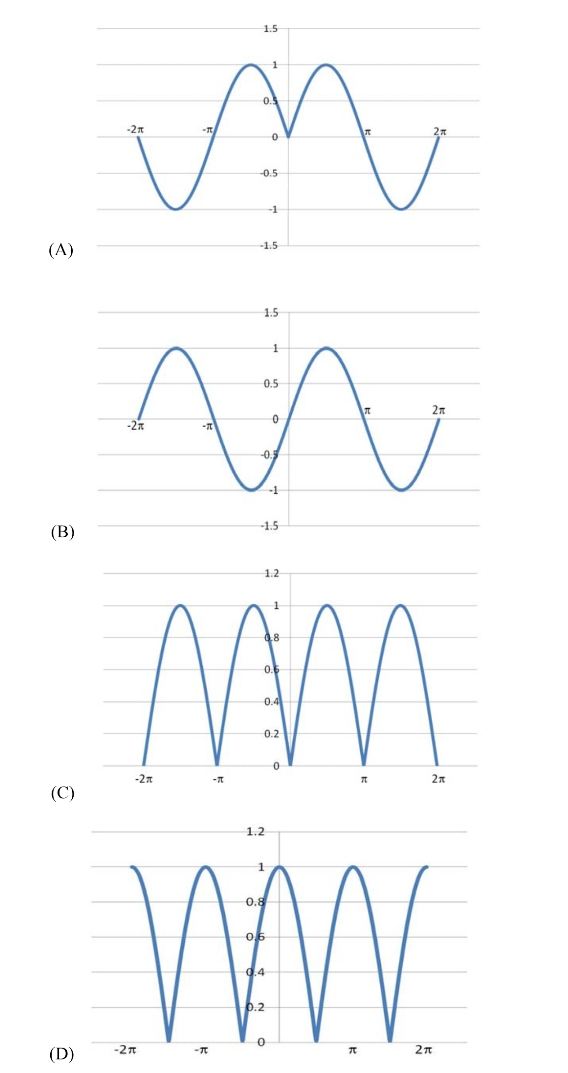
\includegraphics[width=0.31\columnwidth]{figs/qn 10(1).jpg}
    \caption{}
    \label{fig:qn 10.jpg}
\end{figure}

\item Which one of the following is an iterative technique for solving a system of simultaneous linear algebraic equations?
\hfill{\brak{\text{CH 2016}}}
    \begin{enumerate}
    \begin{multicols}{2}
        \item Gauss elimination
        \item Gauss-Jordan
        \item Gauss-Seidel
        \item LU decomposition
        \end{multicols}
    \end{enumerate}

    \item The Laplace transform of $\mathrm{e}^{at} \sin (bt)$ is
    \hfill{\brak{\text{CH 2016}}}
    \begin{enumerate}
    \begin{multicols}{2}
        \item $\dfrac{b}{(s-a)^2 + b^2}$
        \item $\dfrac{(s-a)}{(s-a)^2 + b^2}$
        \item $\dfrac{(s-a)}{(s-a)^2 - b^2}$
        \item $\dfrac{b}{(s-a)^2 - b^2}$
    \end{multicols}
    \end{enumerate}

    \item What are the modulus $(r)$ and argument $(\theta)$ of the complex number $3+4i$ ?
    \hfill{\brak{\text{CH 2016}}}
    \begin{enumerate}
    \begin{multicols}{2}
        \item $r = \sqrt{7}, \quad \theta = \tan^{-1}\left(\dfrac{4}{3}\right)$
        \item $r = \sqrt{7}, \quad \theta = \tan^{-1}\left(\dfrac{3}{4}\right)$
        \item $r = 5, \quad \theta = \tan^{-1}\left(\dfrac{3}{4}\right)$
        \item $r = 5, \quad \theta = \tan^{-1}\left(\dfrac{4}{3}\right)$
        \end{multicols}
    \end{enumerate}

    \item A liquid mixture of ethanol and water is flowing as inlet stream P into a stream splitter. It is split into two streams, Q and R, as shown in the figure below.
    
   \begin{figure}[H]
       \centering
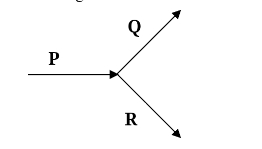
\includegraphics[width=0.25\columnwidth]{figs/qn 4.jpg}
       \caption{}
       \label{fig:qn 14,jpg}
   \end{figure}

    The flowrate of P, containing 30 mass\% of ethanol, is $100 \ \mathrm{kg/h}$. What is the least number of additional specification(s) required to determine the mass flowrates and compositions (mass\%) of the two exit streams?
    \hfill{\brak{\text{CH 2016}}}
    \begin{enumerate}
    \begin{multicols}{4}
        \item $0$
        \item $1$
        \item $2$
        \item $3$
\end{multicols} 
\end{enumerate}

    \item The partial molar enthalpy (in $\mathrm{kJ/mol}$) of species 1 in a binary mixture is given by $\bar{h}_1 = 2 - 60x_2^2 + 100x_1x_2^2$, where $x_1$ and $x_2$ are the mole fractions of species 1 and 2, respectively. The partial molar enthalpy (in $\mathrm{kJ/mol}$, rounded off to the first decimal place) of species 1 at infinite dilution is \underline{\hspace{1cm}}.\hfill{\brak{\text{CH 2016}}}

        \item For a flow through a smooth pipe, the Fanning friction factor $(f)$ is given by $f = m\mathrm{Re}^{-0.2}$ in the turbulent flow regime, where $\mathrm{Re}$ is the Reynolds number and $m$ is a constant. Water flowing through a section of this pipe with a velocity of $1 \ \mathrm{m/s}$ results in a frictional pressure drop of $10 \ \mathrm{kPa}$. What will be the pressure drop across this section (in $\mathrm{kPa}$), when the velocity of water is $2 \ \mathrm{m/s}$?
        \hfill{\brak{\text{CH 2016}}}
        \begin{enumerate}
            \begin{multicols}{4}
            \item $11.5$
            \item $20$
            \item $34.8$
            \item $40$
            \end{multicols}
        \end{enumerate}

        \item In a cyclone separator used for separation of solid particles from a dust laden gas, the separation factor is defined as the ratio of the centrifugal force to the gravitational force acting on the particle. $S_r$ denotes the separation factor at a location (near the wall) that is at a radial distance $r$ from the centre of the cyclone. Which one of the following statements is INCORRECT?
        \hfill{\brak{\text{CH 2016}}}
        \begin{enumerate}
            \item $S_r$ depends on mass of the particle
            \item $S_r$ depends on the acceleration due to gravity
            \item $S_r$ depends on tangential velocity of the particle
            \item $S_r$ depends on the radial location $(r)$ of the particle
        \end{enumerate}

    \item A vertical cylindrical vessel has a layer of kerosene (of density $800 \, \text{kg/m}^3$) over a layer of water (of density $1000 \, \text{kg/m}^3$). L-shaped glass tubes are connected to the column $30 \, \text{cm}$ apart. The interface between the two layers lies between the two points at which the L-tubes are connected. The levels (in cm) to which the liquids rise in the respective tubes are shown in the figure below.

\begin{figure}[H]
    \centering
    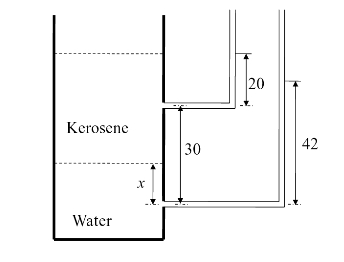
\includegraphics[width=0.5\columnwidth]{figs/qn 8.jpg}
    \caption{}
    \label{fig:qn 18.jpg}
\end{figure}
The distance ($x$ in cm, rounded off to the first decimal place) of the interface from the point at which the lower L-tube is connected is \underline{\hspace{1cm}}.\hfill{\brak{\text{CH 2016}}}

\item A composite wall is made of four different materials of construction in the fashion shown below. The resistance (in K/W) of each of the sections of the wall is indicated in the diagram.
\begin{figure}[H]
    \centering
    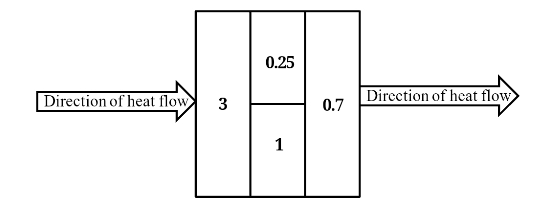
\includegraphics[width=0.5\columnwidth]{figs/qn 9.jpg}
    \caption{}
    \label{fig:qn 19.jpg}
\end{figure}

The overall resistance (in K/W, rounded off to the first decimal place) of the composite wall, in the direction of heat flow, is \underline{\hspace{1cm}}.
\hfill{\brak{\text{CH 2016}}}

\item Steam at $100^\circ\text{C}$ is condensing on a vertical steel plate. The condensate flow is laminar. The average Nusselt numbers are $\text{Nu}_1$ and $\text{Nu}_2$, when the plate temperatures are $10^\circ\text{C}$ and $55^\circ\text{C}$, respectively. Assume the physical properties of the fluid and steel to remain constant within the temperature range of interest. Using Nusselt equations for film-type condensation, what is the value of the ratio $\frac{\text{Nu}_2}{\text{Nu}_1}$?
\hfill{\brak{\text{CH 2016}}}
\begin{enumerate}
\begin{multicols}{4}
\item $0.5$
\item $0.84$
\item $1.19$
\item $1.41$
\end{multicols}
\end{enumerate}

\item A binary liquid mixture of benzene and toluene contains $20 \, \text{mol}\%$ of benzene. At $350 \, \text{K}$ the vapour pressures of pure benzene and pure toluene are $92 \, \text{kPa}$ and $35 \, \text{kPa}$, respectively. The mixture follows Raoult's law. The equilibrium vapour phase mole fraction (rounded off to the second decimal place) of benzene in contact with this liquid mixture at $350 \, \text{K}$ is \underline{\hspace{1cm}}.
\hfill{\brak{\text{CH 2016}}}

\item Match the dimensionless numbers in Group-1 with the ratios in Group-2.

\[\begin{array}{cc}\text{Group-1} & \text{Group-2} \\\hline\text{P} \quad \text{Biot number} & \text{I} \quad \text{buoyancy force} \\\text{Q} \quad \text{Schmidt number} & \text{II} \quad \frac{\text{viscous force}}{\text{internal thermal resistance of a solid}} \\\text{R} \quad \text{Grashof number} & \text{III} \quad \frac{\text{momentum diffusivity}}{\text{mass diffusivity}} \\\end{array}\]
\hfill{\brak{\text{CH 2016}}}
\begin{enumerate}
\begin{multicols}{2}
\item P-II, Q-I, R-III
\item P-I, Q-III, R-II
\item P-III, Q-I, R-II
\item P-II, Q-III, R-I
\end{multicols}
\end{enumerate}

\item For what value of Lewis number, the wet-bulb temperature and adiabatic saturation temperature are nearly equal?
\hfill{\brak{\text{CH 2016}}}
\begin{enumerate}
\begin{multicols}{4}
\item $0.33$
\item $0.5$
\item $1$
\item $2$
\end{multicols}
\end{enumerate}

\item For a non-catalytic homogeneous reaction $\mathrm{A} \rightarrow \mathrm{B}$, the rate expression at $300 \, \mathrm{K}$ is 
$-r_A \, (\mathrm{mol} \, \mathrm{m}^{-3} \, \mathrm{s}^{-1}) = \frac{10C_A}{1+5C_A}$ where $C_A$ is the concentration of A (in $\mathrm{mol/m}^3$). Theoretically, the upper limit for the magnitude of the reaction rate ($-r_A$ in $\mathrm{mol} \, \mathrm{m}^{-3} \, \mathrm{s}^{-1}$, rounded off to the first decimal place) at $300 \, \mathrm{K}$ is \underline{\hspace{1cm}}
\hfill{\brak{\text{CH 2016}}}

\item The variations of the concentrations ($C_A$, $C_B$ and $C_S$) for three species (A, R and S) with time, in an isothermal homogeneous batch reactor are shown in the figure below.
\begin{figure}[H]
    \centering
    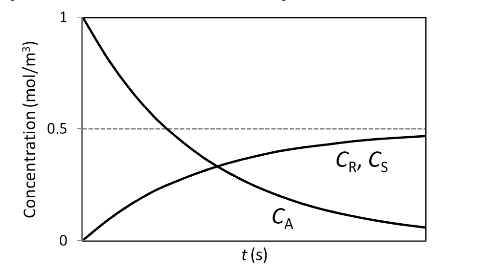
\includegraphics[width=0.5\columnwidth]{figs/qn 15.jpg}
    \caption{}
    \label{fig:qn 15.jpg}
\end{figure}
Select the reaction scheme that correctly represents the above plot. The numbers in the reaction schemes shown below, represent the first order rate constants in unit of $\text{s}^{-1}$.
\hfill{\brak{\text{CH 2016}}}
\begin{figure}[H]
    \centering
    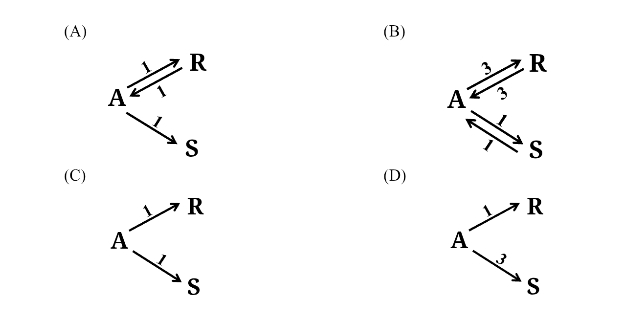
\includegraphics[width=0.5\columnwidth]{figs/qn 15 opt.jpg}
    \caption{}
    \label{fig:qn.15 opt.jpg}
\end{figure}
\item Hydrogen iodide decomposes through the reaction $2\text{HI} = \text{H}_2 + \text{I}_2$. The value of the universal gas constant is $8.314 \text{ J mol}^{-1} \text{ K}^{-1}$. The activation energy for the forward reaction is $184000 \text{ J mol}^{-1}$. The ratio (rounded off to the first decimal place) of the forward reaction rate at $600 \text{ K}$ to that at $550 \text{ K}$ is \underline{\hspace{1cm}}.
\hfill{\brak{\text{CH 2016}}}

\item Match the instruments in Group-1 with process variables in Group-2.
\begin{center}
\begin{tabular}{c|c}
Group-1 & Group-2 \\
\hline
P. Conductivity meter & I. Flow \\
Q. Turbine meter & II. Pressure \\
R. pH electrode & III. Composition \\
\end{tabular}
\end{center}
\hfill{\brak{\text{CH 2016}}}
\begin{enumerate}
\begin{multicols}{2}
\item P-II, Q-III, R-I
\item P-II, Q-I, R-III
\item P-III, Q-II, R-I
\item P-III, Q-I, R-II
\end{multicols}
\end{enumerate}

\item What is the order of response exhibited by a U-tube manometer?
\hfill{\brak{\text{CH 2016}}}
\begin{enumerate}
\begin{multicols}{2}
\item Zero order
\item First order
\item Second order
\item Third order
\end{multicols}
\end{enumerate}

\item A system exhibits inverse response for a unit step change in the input. Which one of the following statements must necessarily be satisfied?
\hfill{\brak{\text{CH 2016}}}
\begin{enumerate}
\item The transfer function of the system has at least one negative pole
\item The transfer function of the system has at least one positive pole
\item The transfer function of the system has at least one negative zero
\item The transfer function of the system has at least one positive zero
\end{enumerate}

\item Two design options for a distillation system are being compared based on the total annual cost. Information available is as follows:
\begin{center}
\begin{tabular}{c|c|c}
& Option P & Option Q \\
\hline
Installed cost of the system (Rs in lakhs) & 150 & 120 \\
Cost of cooling water for condenser (Rs lakhs/year) & 6 & 8 \\
Cost of steam for reboiler (Rs lakhs/year) & 16 & 20 \\
\end{tabular}
\end{center}
The annual fixed charge amounts to $12\%$ of the installed cost. Based on the above information, what is the total annual cost (Rs in lakhs/year) of the better option?
\hfill{\brak{\text{CH 2016}}}
\begin{enumerate}
\begin{multicols}{4}
\item $40$
\item $42.4$
\item $92$
\item $128$
\end{multicols}
\end{enumerate}

\item Standard pipes of different schedule numbers and standard tubes of different BWG numbers are available in market. For a pipe / tube for a given nominal diameter, which one of the following statements is TRUE?
\hfill{\brak{\text{CH 2016}}}
\begin{enumerate}
\item Wall thickness increases with increase in both the schedule number and the BWG number
\item Wall thickness increases with increase in the schedule number and decreases with increase in the BWG number
\item Wall thickness decreases with increase in both the schedule number and the BWG number
\item Neither the schedule number, nor the BWG number has any relation to wall thickness
\end{enumerate}

\item Terms used in engineering economics have standard definitions and interpretations. Which one of the following statements is INCORRECT?
\hfill{\brak{\text{CH 2016}}}
\begin{enumerate}
\item The profitability measure `return on investment' does not consider the time value of money
\item A cost index is an index value for a given time showing the cost at that time relative to a certain base time
\item The `six-tenths factor rule' is used to estimate the cost of an equipment from the cost of a similar equipment with a different capacity
\item Payback period is calculated based on the payback time for the sum of the fixed and the working capital investment
\end{enumerate}

\item India has no elemental sulphur deposits that can be economically exploited. In India, which one of the following industries produces elemental sulphur as a by-product?
\hfill{\brak{\text{CH 2016}}}
\begin{enumerate}
\item Coal carbonisation plants
\item  Petroleum refineries
\item  Paper and pulp industries
\item  Iron and steel making plants
\end{enumerate}

\item Two paper pulp plants P and Q use the same quality of bamboo as a raw material. The chemicals used in their digester are as follows:
\[\begin{array}{c|c|c}& \text{Plant P} & \text{Plant Q} \\\hline\text{NaOH} & \text{Yes} & \text{No} \\\text{Na}_2\text{S} & \text{Yes} & \text{No} \\\text{Na}_2\text{CO}_3 & \text{Yes} & \text{Yes} \\\text{NaHCO}_3 & \text{No} & \text{Yes} \\\text{Na}_2\text{SO}_3 & \text{No} & \text{Yes} \\\end{array}\]
Which one of the following statements is CORRECT?
\hfill{\brak{\text{CH 2016}}}
\begin{enumerate}
\item Plant P and Plant Q both use the Sulfite process
\item Plant P and Plant Q both use the Kraft process
\item Plant P uses Sulfite process
\item Plant P uses Kraft process
\end{enumerate}

\item Match the industrial processes in Group-1 with the catalyst materials in Group-2.
\[\begin{array}{c|l}\text{Group-1} & \text{Group-2} \\\hline\text{P: Ethylene polymerisation} & \text{I: Nickel} \\\text{Q: Petroleum feedstock cracking} & \text{II: Vanadium pentoxide} \\\text{R: Oxidation of SO}_2 \text{ to SO}_3 & \text{III: Zeolite} \\\text{S: Hydrogenation of oil} & \text{IV: Aluminium triethyl with titanium chloride promoter}\end{array}\]
\hfill{\brak{\text{CH 2016}}}
\begin{enumerate}
\begin{multicols}{4}
\item P-IV, Q-III, R-II, S-I
\item P-I, Q-IV, R-III, S-II
\item P-I, Q-II, R-III, S-IV
\item P-II, Q-III, R-IV, S-I
\end{multicols}
\end{enumerate}
\section*{Q. 36--Q. 55 carry two mark each.}

\item A set of simultaneous linear algebraic equations is represented in a matrix form as shown below.
\[\begin{bmatrix}0 & 0 & 0 & 4 & 13 \\2 & 5 & 2 & 10 & 0 \\0 & 0 & 2 & 5 & 3 \\0 & 0 & 4 & 5 & 0 \\2 & 3 & 2 & 1 & 5\end{bmatrix}\begin{bmatrix}x_1 \\x_2 \\x_3 \\x_4 \\x_5\end{bmatrix}=\begin{bmatrix}46 \\161 \\61 \\30 \\81\end{bmatrix}\]
The value (rounded off to the nearest integer) of $x_3$ is \underline{\hspace{1cm}}.

\item What is the solution for the second order differential equation $\dfrac{d^2y}{dx^2} + y = 0$, with the initial conditions $y\big|{x=0} = 5$ and $\dfrac{dy}{dx}\bigg|{x=0} = 10$ ?
\hfill{\brak{\text{CH 2016}}}
\begin{enumerate}
\begin{multicols}{2}
\item $y=5+10\sin x$
\item $y=5\cos x-5\sin x$
\item $y=5\cos x+10x$
\item $y=5\cos x+10\sin x$
\end{multicols}
\end{enumerate}

\item The model $y = mx^2$ is to be fit to the data given below.
\[\begin{array}{c|c|c|c}x & 1 & \sqrt{2} & \sqrt{3} \\\hliney & 2 & 5 & 8\end{array}\]
Using linear regression, the value (rounded off to the second decimal place) of $m$ is \underline{\hspace{1cm}}.
\hfill{\brak{\text{CH 2016}}}

\item The Lagrange mean-value theorem is satisfied for $f (x) = x^3 +5$, in the interval $(1,4)$ at a value (rounded off to the second decimal place) of $x$ equal to \underline{\hspace{1cm}}.
\hfill{\brak{\text{CH 2016}}}

\item Values of $f (x)$ in the interval $[0, 4]$ are given below.
\[\begin{array}{c|c|c|c|c|c}x & 0 & 1 & 2 & 3 & 4 \\\hlinef(x) & 3 & 10 & 21 & 36 & 55\end{array}\]
Using Simpson's $1/3$ rule with a step size of 1, the numerical approximation (rounded off to the second decimal place) of $\int_{0}^{4} f(x) dx$ is \underline{\hspace{1cm}}.
\hfill{\brak{\text{CH 2016}}}

\item A jacketed stirred tank with a provision for heat removal is used to mix sulphuric acid and water in a steady state flow process. $\text{H}_2\text{SO}_4 (\ell)$ enters at a rate of $4 \text{ kg/h}$ at $25^\circ\text{C}$ and $\text{H}_2\text{O} (\ell)$ enters at a rate of $6 \text{ kg/h}$ at $10^\circ\text{C}$. The following data are available:

Specific heat capacity of water $= 4.2 \text{ kJ kg}^{-1} \text{K}^{-1}$.

Specific heat capacity of aqueous solution of $40 \text{ mass}\% \text{ H}_2\text{SO}_4 = 2.8 \text{ kJ (kg solution)}^{-1} \text{K}^{-1}$.

Assume the specific heat capacities to be independent of temperature.

Based on reference states of $\text{H}_2\text{SO}_4 (\ell)$ and $\text{H}_2\text{O} (\ell)$ at $25^\circ\text{C}$, the heat of mixing for aqueous solution of $40 \text{ mass}\% \text{ H}_2\text{SO}_4 = -650 \text{ kJ (kg solution)}^{-1}$.

If the mixed stream leaves at $40^\circ\text{C}$, what is the rate of heat removal (in $\text{kJ/h}$)?
\hfill{\brak{\text{CH 2016}}}
\begin{enumerate}
\begin{multicols}{4}
\item $1802$
\item $2558$
\item $5702$
\item $6458$
\end{multicols}
\end{enumerate}

\item An ideal gas is adiabatically and irreversibly compressed from 3 bar and 300 K to 6 bar in a closed system. The work required for the irreversible compression is 1.5 times the work that is required for reversible compression from the same initial temperature and pressure to the same final pressure. The molar heat capacity of the gas at constant volume is $30 \text{ J mol}^{-1} \text{K}^{-1}$ (assumed to be independent of temperature); universal gas constant, $R = 8.314 \text{ J mol}^{-1} \text{K}^{-1}$; ratio of molar heat capacities is $1.277$. The temperature (in K, rounded off to the first decimal place) of the gas at the final state in the irreversible compression case is \underline{\hspace{1cm}}.\hfill{\brak{\text{CH 2016}}}

\item A gas obeying the Clausius equation of state is isothermally compressed from $5 \, \text{MPa}$ to $15 \, \text{MPa}$ in a closed system at $400 \, \text{K}$. The Clausius equation of state is $P = \frac{RT}{v - b(T)}$ where $P$ is the pressure, $T$ is the temperature, $v$ is the molar volume and $R$ is the universal gas constant. The parameter $b$ in the above equation varies with temperature as $b(T) = b_0 + b_1 T$ with $b_0 = 4 \times 10^{-6} \, \text{m}^3 \text{mol}^{-1}$ and $b_1 = 1.35 \times 10^{-7} \, \text{m}^3 \text{mol}^{-1} \text{K}^{-1}$. The effect of pressure on the molar enthalpy ($h$) at a constant temperature is given by $h - h^{IG} = \int v - T \left( \frac{\partial v}{\partial T} \right)P dP$. Let $h_i$ and $h_f$ denote the initial and final molar enthalpies, respectively. The change in the molar enthalpy $h_f - h_i$ (in $\text{J} \, \text{mol}^{-1}$, rounded off to the first decimal place) for this process is \underline{\hspace{1cm}}.\hfill{\brak{\text{CH 2016}}}

\item A binary system at a constant pressure with species `$1$' and `' and `$2$' is described by the two-suffix Margules equation, $g^E = A x_1 x_2$, where $g^E$ is the molar excess Gibbs free energy, $R$ is the universal gas constant, $T$ is the temperature and $x_1$, $x_2$ are the mole fractions of species 1 and 2, respectively.

At a temperature $T$, $g_1 = A/2$ and $g_2 = A/2$, where $g_1$ and $g_2$ are the molar Gibbs free energies of pure species 1 and 2, respectively. At the same temperature, $g$ represents the molar Gibbs free energy of the mixture. For a binary mixture with $40 \, \text{mole} \, \%$ of species 1, the value (rounded off to the second decimal place) of $\frac{g}{RT}$ is \underline{\hspace{1cm}}.\hfill{\brak{\text{CH 2016}}}

\item  Water (density$=1000 \, \text{kg} \, \text{m}^{-3}$) is pumped at a rate of $36 \, \text{m}^3/\text{h}$, from a tank $2 \, \text{m}$ below the pump, to an overhead pressurized vessel $10 \, \text{m}$ above the pump. The pressure values at the point of suction from the bottom tank and at the discharge point to the overhead vessel are $120 \, \text{kPa}$ and $240 \, \text{kPa}$, respectively. All pipes in the system have the same diameter. Take acceleration due to gravity, $g = 10 \, \text{m} \, \text{s}^{-2}$. Neglecting frictional losses, what is the power (in $\text{kW}$) required to deliver the fluid?
\hfill{\brak{\text{CH 2016}}}
\begin{enumerate}
\begin{multicols}{4}
\item $1.2$ 
\item $2.4$ 
\item $3.6$ 
\item $4.8$
\end{multicols}
\end{enumerate}

\item An agitated cylindrical vessel is fitted with baffles and flat blade impellers. The power number for this system is given by $N_p = \frac{P}{\rho n^3 D^5}$ where $P$ is the power consumed for the mixing, $\rho$ is the density of the fluid, $n$ is the speed of the impeller and $D$ is the diameter of the impeller. The diameter of the impeller is $1/3^{\text{rd}}$ diameter of the tank and the height of liquid level is equal to tank diameter. The impeller speed to achieve the desired degree of mixing is 4 rpm. In a scaled up design, the linear dimensions of the equipment are to be doubled, holding the power input per unit volume constant. Assuming the liquid to be Newtonian and $N_p$ to be independent of Reynolds number, what is the impeller speed (in rpm) to achieve the same degree of mixing in the scaled up vessel?
\hfill{\brak{\text{CH 2016}}}
\begin{enumerate}
\begin{multicols}{4}
\item $0.13$
\item $1.26$
\item $2.52$
\item $3.82$
\end{multicols}
\end{enumerate}

\item Consider a rigid solid sphere falling with a constant velocity in a fluid. The following data are known at the conditions of interest: viscosity of the fluid = $0.1$ Pa s, acceleration due to gravity = $10$ m s$^{-2}$, density of the particle = $1180$ kg m$^{-3}$ and density of the fluid = $1000$ kg m$^{-3}$. The diameter (in mm, rounded off to the second decimal place) of the largest sphere that settles in the Stokes' law regime (Reynolds number $\leq 0.1$), is \underline{\hspace{1cm}}.\hfill{\brak{\text{CH 2016}}}

\item The characteristics curve (Head - Capacity - relationship) of a centrifugal pump is represented by the equation $\Delta H_{\text{pump}} = 43.8 - 0.19Q$, where $\Delta H_{\text{pump}}$ is the head developed by the pump (in m) and $Q$ is the flowrate (in m$^3$/h) through the pump. This pump is to be used for pumping water through a horizontal pipeline. The frictional head loss $\Delta H_{\text{piping}}$ (in m) is related to the water flowrate $Q_L$ (in m$^3$/h) by the equation $\Delta H_{\text{piping}} = 0.0135Q_L^2 + 0.045Q_L$. The flowrate (in m$^3$/h, rounded off to the first decimal place) of water pumped through the above pipeline, is \underline{\hspace{1cm}}.
\hfill{\brak{\text{CH 2016}}}

\item Water flows through a smooth circular pipe under turbulent conditions. In the viscous sub-layer, the velocity varies linearly with the distance from the wall. The Fanning friction factor is defined as, $f = \frac{\tau_w}{\rho \bar{u}^2/2}$ where $\tau_w$ is the shear stress at the wall of the pipe, $\rho$ is the density of the fluid and $\bar{u}$ is the average velocity in the pipe. Water (density = $1000$ kg m$^{-3}$, viscosity = $1 \times 10^{-3}$ kg m$^{-1}$ s$^{-1}$) flows at an average velocity of $1$ m s$^{-1}$ through the pipe. For this flow condition, the friction factor $f$ is $0.005$. At a distance of $0.05$ mm from the wall of the pipe (in the viscous sub-layer), the velocity (in m s$^{-1}$, rounded off to the third decimal place), is \underline{\hspace{1cm}}.\hfill{\brak{\text{CH 2016}}}

\item In a 1-1 pass shell and tube exchanger, steam is condensing in the shell side at a temperature $(T_s)$ of $135^\circ\text{C}$ and the cold fluid is heated from a temperature $(T_1)$ of $20^\circ\text{C}$ to a temperature $(T_2)$ of $90^\circ\text{C}$. The energy balance equation for this heat exchanger is

\[\ln \frac{T_s - T_1}{T_s - T_2} = \frac{UA}{\dot{m}c_p}\]

where $U$ is the overall heat transfer coefficient, $A$ is the heat transfer area, $\dot{m}$ is the mass flow rate of the cold fluid and $c_p$ is its specific heat. Tube side fluid is in a turbulent flow and the heat transfer coefficient can be estimated from the following equation:

\[\text{Nu} = 0.023 (\text{Re})^{0.8}(\text{Pr})^{0.3}\]

where Nu is the Nusselt number, Re is the Reynolds number and Pr is the Prandtl number. The condensing heat transfer coefficient in the shell side is significantly higher than the tube side heat transfer coefficient. The resistance of the wall to heat transfer is negligible. If only the mass flow rate of the cold fluid is doubled, what is the outlet temperature (in $^\circ\text{C}$) of the cold fluid at steady state?
\hfill{\brak{\text{CH 2016}}}
\begin{enumerate}
\begin{multicols}{4}
\item $80.2$
\item $84.2$
\item $87.4$
\item $88.6$
\end{multicols}
\end{enumerate}

\item In an experimental setup, mineral oil is filled in between the narrow gap of two horizontal smooth plates. The setup has arrangements to maintain the plates at desired uniform temperatures. At these temperatures, ONLY the radiative heat flux is negligible. The thermal conductivity of the oil does not vary perceptibly in this temperature range. Consider four experiments at steady state under different experimental conditions, as shown in the figure below. The figure shows plate temperatures and the heat fluxes in the vertical direction.
\begin{figure}[H]
    \centering
    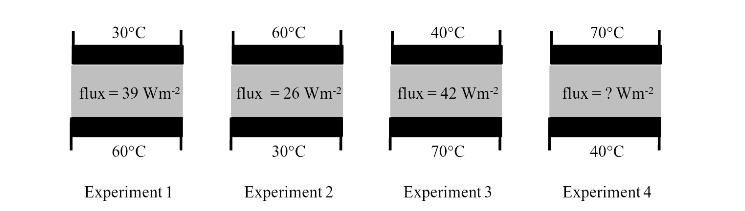
\includegraphics[width=0.5\columnwidth]{figs/qn 41.jpg}
    \caption{}
    \label{fig:qn 51.jpg}
\end{figure}
What is the steady state heat flux (in W/m$^2$) with the top plate at $70^\circ$C and the bottom plate at $40^\circ$C?
\hfill{\brak{\text{CH 2016}}}
\begin{enumerate}
\begin{multicols}{4}
    \item $26$
    \item $39$
    \item $42$
    \item $63$
    \end{multicols}
\end{enumerate}

\item The space between two hollow concentric spheres of radii $0.1$ m and $0.2$ m is under vacuum. Exchange of radiation (uniform in all directions) occurs only between the outer surface ($S_1$) of the smaller sphere and the inner surface ($S_2$) of the larger sphere. The fraction (rounded off to the second decimal place) of the radiation energy leaving $S_2$, which reaches $S_1$ is \underline{\hspace{1cm}}.\hfill{\brak{\text{CH 2016}}}

\item A binary distillation column is to be designed using McCabe Thiele method. The distillate contains $90$ mol\% of the more volatile component. The point of intersection of the $q$-line with the equilibrium curve is $(0.5, 0.7)$. The minimum reflux ratio (rounded off to the first decimal place) for this operation is \underline{\hspace{1cm}}.\hfill{\brak{\text{CH 2016}}}

\item Solute C is extracted in a batch process from its homogenous solution of A and C, using solvent B. The combined composition of the feed and the extracting solvent is shown in the figure below as point M, along with the tie line passing through it. The ends of the tie line are on the equilibrium curve.
\begin{figure}[H]
    \centering
    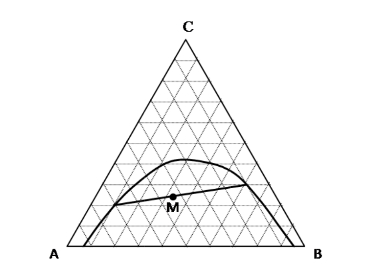
\includegraphics[width=0.5\columnwidth]{figs/qn 44.jpg}
    \caption{}
    \label{fig:qn 54.jpg}
\end{figure}
What is the selectivity for C?
\hfill{\brak{\text{CH 2016}}}
\begin{enumerate}
\begin{multicols}{4}
\item $3.5$
\item $7$
\item $10.5$
\item $21$
\end{multicols}
\end{enumerate}
\item At $30^\circ\text{C}$, the amounts of acetone adsorbed at partial pressures of 10 and 100 mmHg are 0.1 and 0.4 kg acetone/kg activated carbon, respectively. Assume Langmuir isotherm describes the adsorption of acetone on activated carbon. What is the amount of acetone adsorbed (in kg per kg of activated carbon) at a partial pressure of 50 mmHg and $30^\circ\text{C}$?
\hfill{\brak{\text{CH 2016}}}
\begin{enumerate}
\begin{multicols}{4}
\item $0.23$
\item $0.25$
\item $0.30$
\item $0.35$
\end{multicols}
\end{enumerate}

\item Consider the following two cases for a binary mixture of ideal gases A and B under steady state conditions. In Case 1, the diffusion of A occurs through non-diffusing B. In Case 2, equimolar counter diffusion of A and B occurs. In both the cases, the total pressure is 100 kPa and the partial pressures of A at two points separated by a distance of 10 mm are 10 kPa and 5 kPa. Assume that the Fick's first law of diffusion is applicable. What is the ratio of molar flux of A in Case 1 to that in Case 2?
\hfill{\brak{\text{CH 2016}}}
\begin{enumerate}
\begin{multicols}{4}
    \item $0.58$
    \item $1.08$
    \item $1.58$
    \item $2.18$
    \end{multicols}
\end{enumerate}

\item The liquid phase reversible reaction $A \rightleftharpoons B$ is carried out in an isothermal CSTR operating under steady state conditions. The inlet stream does not contain B and the concentration of A in the inlet stream is 10 mol/lit. The concentrations of A at the reactor exit, for residence times of 1 s and 5 s are 8 mol/lit and 5 mol/lit, respectively. Assume the forward and backward reactions are elementary following the first order rate law. Also assume that the system has constant molar density. The rate constant of the forward reaction (in s$^{-1}$, rounded off to the third decimal place) is \underline{\hspace{1cm}}.\hfill{\brak{\text{CH 2016}}}

\item A liquid phase irreversible reaction $A \rightarrow B$ is carried out in an adiabatic CSTR operating under steady state conditions. The reaction is elementary and follows the first order rate law. For this reaction, the figure below shows the conversion $(X_{A})$ of A as a function of temperature $(T)$ for different values of the rate of reaction $(-r_{A}$ in $\text{mol m}^{-3}\text{s}^{-1} )$ denoted by the numbers to the left of each curve. This figure can be used to determine the rate of the reaction at a particular temperature, for a given conversion of A.

\begin{figure}[H]
    \centering
    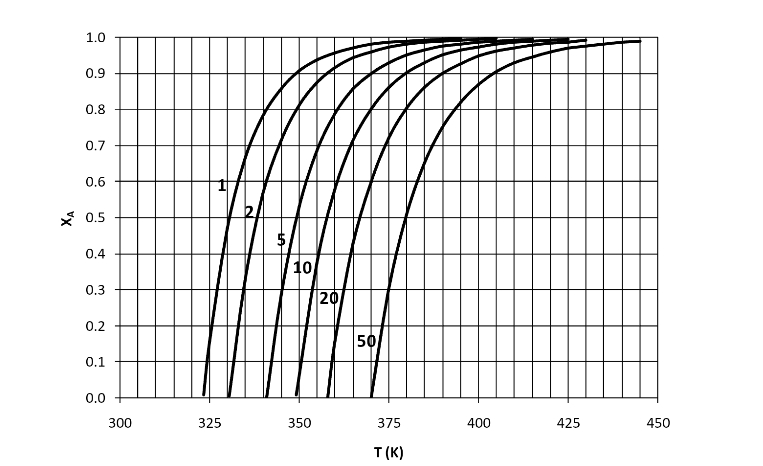
\includegraphics[width=0.5\columnwidth]{figs/qn 48.jpg}
    \caption{}
    \label{fig:qn 58.jpg}
\end{figure}
The inlet stream does not contain B and the concentration of A in the inlet stream is $5 \, \text{mol/m}^3$. The molar feed rate of A is $100 \, \text{mol/s}$. A steady state energy balance for this CSTR results in the following relation: $T = 350 + 25X_A$ where $T$ is the temperature (in K) of the exit stream and $X_A$ is the conversion of A in the CSTR. For an exit conversion of $80 \, \%$ of A, the volume (in $\text{m}^3$, rounded off to the first decimal place) of CSTR required is 
 \underline{\hspace{1cm}}.\hfill{\brak{\text{CH 2016}}}

\item A porous pellet with Pt dispersed in it is used to carry out a catalytic reaction. Following two scenarios are possible.

Scenario 1: Pt present throughout the pores of the pellet is used for catalyzing the reaction. \\
Scenario 2: Pt present only in the immediate vicinity of the external surface of the pellet is used for catalyzing the reaction.

At a large value of Thiele modulus, which one of the following statements is \textbf{TRUE}?
\hfill{\brak{\text{CH 2016}}}
\begin{enumerate}
\item Since the reaction rate is much greater than the diffusion rate, Scenario 1 occurs
\item Since the reaction rate is much greater than the diffusion rate, Scenario 2 occurs
\item Since the reaction rate is much lower than the diffusion rate, Scenario 1 occurs
\item Since the reaction rate is much lower than the diffusion rate, Scenario 2 occurs
\end{enumerate}

\item A CSTR has a long inlet pipe. A tracer is injected at the entrance of the pipe. The E-curve obtained at the exit of the CSTR is shown in the figure below.
\begin{figure}[H]
    \centering
    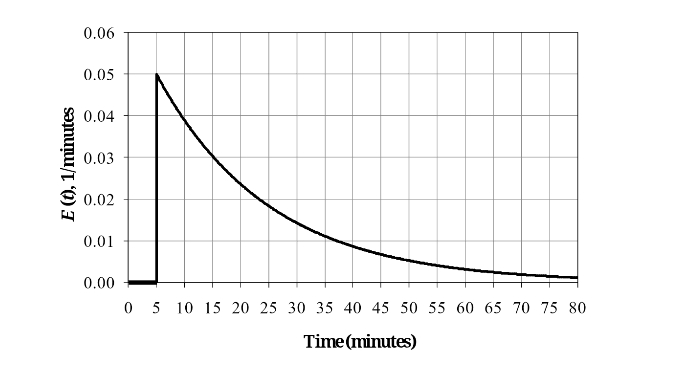
\includegraphics[width=0.5\columnwidth]{figs/qn 50.jpg}
    \caption{}
    \label{fig:qn 60.jpg}
\end{figure}
Assuming plug flow in the inlet pipe, the ratio (rounded off to the second decimal place) of the volume of the pipe to that of the CSTR is \underline{\hspace{1cm}}.
\hfill{\brak{\text{CH 2016}}}

\item A liquid flows through an ``equal percentage'' valve at a rate of $2 \, \text{m}^3/\text{h}$ when the valve is $10\%$ open. When the valve opens to $20\%$ the flowrate increases to $3 \, \text{m}^3/\text{h}$. Assume that the pressure drop across the valve and the density of the liquid remain constant. When the valve opens to $50\%$, the flowrate (in $\text{m}^3/\text{h}$, rounded off to the second decimal place) is \underline{\hspace{1cm}}.
\hfill{\brak{\text{CH 2016}}}

\item A PI controller with integral time constant of $0.1$ min is to be designed to control a process with transfer function
\[G_p(s) = \frac{10}{s^2 + 2s + 100}\]
Assume the transfer functions of the measuring element and the final control element are both unity ($G_m = 1, G_f = 1$). The gain (rounded off to the first decimal place) of the controller that will constitute the critical condition for stability of the PI feedback control system is \underline{\hspace{1cm}}.
\hfill{\brak{\text{CH 2016}}}

\item For a unit step input, the response of a second order system is
\[y(t) = K_p \left[ 1 - \frac{1}{\sqrt{1-\zeta^2}} e^{\frac{-\zeta t}{\tau}} \sin \left( \frac{\sqrt{1-\zeta^2}}{\tau} t + \phi \right) \right]\]
where, $K_p$ is the steady state gain, $\zeta$ is the damping coefficient, $\tau$ is the natural period of oscillation and $\phi$ is the phase lag. The overshoot of the system is $\exp \left( \frac{-\pi\zeta}{\sqrt{1-\zeta^2}} \right)$. For a unit step input, the response of the system from an initial steady state condition at $t = 0$ is shown in the figure below.
\begin{figure}[H]
    \centering
    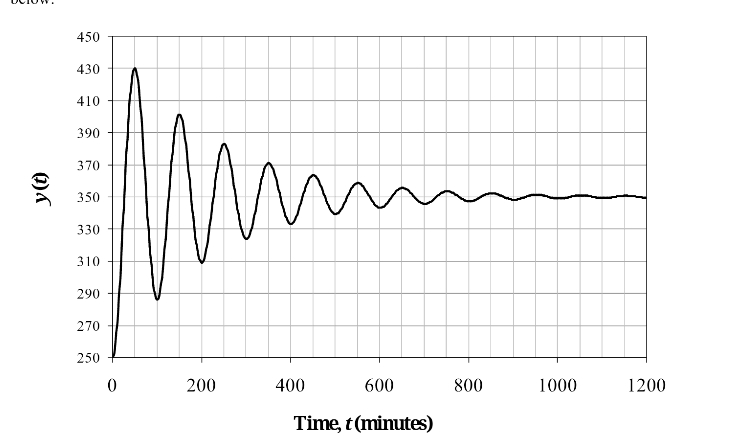
\includegraphics[width=0.5\columnwidth]{figs/qn 53.jpg}
    \caption{}
    \label{fig:qn 53.jpg}
\end{figure}
What is the natural period of oscillation (in seconds) of the system?
\hfill{\brak{\text{CH 2016}}}
\begin{enumerate}
\begin{multicols}{4}
    \item $15.9$
    \item $50$
    \item $63.2$
    \item $100$
\end{multicols}
\end{enumerate}

\item A vertical cylindrical tank with a flat roof and bottom is to be constructed for storing $150 \, \text{m}^3$ of ethylene glycol. The cost of material and fabrication for the tank wall is Rs $6000$ per $\text{m}^2$ and the same for the roof and the tank bottom are Rs $2000$ and Rs $4000$ per $\text{m}^2$, respectively. The cost of accessories, piping and instruments can be taken as $10\%$ of the cost of the wall. $10\%$ of the volume of the tank needs to be kept free as vapour space above the liquid storage. What is the optimum diameter (in m) for the tank?
\hfill{\brak{\text{CH 2016}}}
\begin{enumerate}
\begin{multicols}{4}
    \item $3.5$
    \item $3.9$
    \item $7.5$
    \item $7.8$
    \end{multicols}
    \end{enumerate}
\item A catalytic reforming plant produces hydrogen and benzene from cyclohexane by de-hydro aromatisation. In order to increase the production of hydrogen, the owner plans to change the process to steam reforming of the same feedstock that produces hydrogen and carbon dioxide. Stoichiometrically, what is the maximum ratio of pure hydrogen produced in the proposed process to that in the existing process?
\hfill{\brak{\text{CH 2016}}}
\begin{enumerate}
\begin{multicols}{4}
    \item $1$
    \item $2$
    \item $5$
    \item $6$
    \end{multicols}
\end{enumerate}
    \centering
\textbf{END OF THE QUESTION PAPER}
\end{enumerate}

\end{document}